\documentclass[sprache=english,fontsize=11,hausschrift=times,betreuerform=tabelle]{TUBAFarbeiten}
\usepackage[utf8]{inputenc}
\usepackage[T1]{fontenc}
\usepackage[export]{adjustbox}
\usepackage{csquotes}
\usepackage{hyperref}
\usepackage{amsmath}
\usepackage{graphicx}
\usepackage{subcaption}
\usepackage[backend=biber,sorting=none]{biblatex}
% \bibliography{References}
\TUBAFTitel{Image convolution with MPI}
\TUBAFUntertitel{Programming Project | Winter Semester 2020-2021}
\TUBAFAutor{Venkata Mukund Kashyap Yedunuthala}
\TUBAFStudiengang{Computational Materials Science}
\TUBAFMatrikel{65\,163}
\TUBAFDatumfs{\today}
\begin{document}
\maketitle[intertext={A report on}]
\TUBAFErklaerungsseite
\tableofcontents
\listoffigures
\clearpage
\section{Introduction}
This programming project focuses on convolution of a grayscale image with the following three convolution 
kernels:
\begin{itemize}
    \item Blurring
    \item Sharpening
    \item Edge Detection
\end{itemize}

The program thus developed has been implemented in parallel with Message Passing Interface (MPI) 
using C++ programming language in the high performance computing cluster of TU Bergakademie Freiberg. 

\subsection*{Format of the grayscale image}
The images provided are in Netpbm grayscale image format. Quoted as "the lowest common denominator grayscale 
file format," this format had been chosen due to its ease in coding. Unlike the color images consisting of three color channels,
with every pixel displaying the combined information of Red, Green and Blue channels, this format consists of one channel.
The images considered in this project are said to be of 8-bit depth, i.e. the values of the pixels lie within the interval $[0,255]$.
The value 0 describes black, whereas 255 describes white. The images provided within this project are of uncompressed PGM data format. 
Therefore, initially, these values are read into a two-dimensional arrays, which are worked upon. Upon completion, the resultant arrays 
are written to file as per the specifications, which can then be converted to different formats using ImageMagick software. 
\section{Convolution kernels}
Within the context of image processing, a convolution kernel, or a kernel, refers to a matrix that allows manipulation of values of pixel
as per requirements. The procedure, known as convolution, refers to the process of computing a new pixel value from the given pixel value along
with its surrounding pixel values. The kernels are specified below. 

\subsection{Gaussian Blur}
The aim of this kernel is to smoothen an image, or reduce the noise or detail within an image.
specified below. 
$$
    \frac{1}{16}
    \begin{bmatrix}
        1 & 2 & 1 \\ 2 & 4 & 2 \\ 1 & 2 & 1
    \end{bmatrix}
$$
\subsection{Sharpen}
The aim of this kernel is to enhance the sharpness of the image, can be understood to be the opposite of blur.
$$
    \begin{bmatrix}
        0 & -1 & 0 \\ -1 & 5 & -1 \\ 0 & -1 & 0
    \end{bmatrix}
$$
\subsection{Edge Detection}
The aim of this kernel is to identify the edges present in the image. In the context of image processing, an edge can be understood as the collection of 
points where the brightness suddenly changes, or has discontinuities.
$$
\begin{bmatrix}
    -1 & -1 & -1 \\ -1 & 8 & -1 \\ -1 & -1 & -1
\end{bmatrix}
$$

Then, the respective convolution kernel is then applied to a pixel value $I(x,y)$ to obtain a new pixel value $I^*(x,y)$ 
where $(x,y)$ denotes the position in the image. Convolution procedure can be shown in a mathematical format as follows.
$$ I^*(x,y) = \sum_{i=1}^{n}\sum_{i=1}^{n}I(x-i+2,y-j+2)k(i,j) $$ where $k$ represents the chosen 3 x 3 convolution kernel.
An important aspect to note is the treatment of pixel values at the boundaries of the image. In this implementation, these
are treated periodically, i.e. the pixel value at positon $(1,0)$ receives information from $(1,511)$, the opposite border,
in order to finish the computation of new pixel value.

\section{MPI Parallelization and Communication}

For the parallel implementation of this code, MPI library is applied. The pixel values are thus distributed in a way such that each process has its own
chunk of rows of pixel values, including the information belonging to the halo. Here, a halo refers to the rows of pixels indicated by dashed lines in the figure
The figure representing this division can be seen here in Fig.\ref{Fig.1}. The code is then executed on the university's high performance computing cluster and the
times are tabulated against number of processes to assess scalability.
\begin{figure}
    \centering
    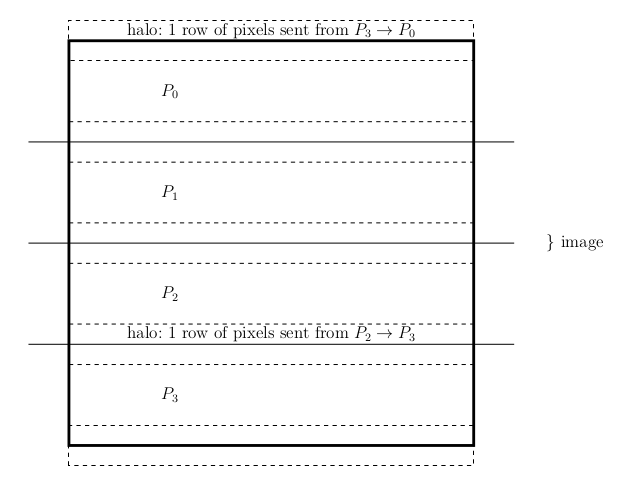
\includegraphics[scale=0.5]{inputs/MPI.png}
    \caption{Distribution of data between processes}
    \label{Fig.1}
\end{figure}
\newpage
\section{Results}
At the beginning, the results belonging to the 512 x 512 image are presented. Fig.\ref{Fig.2a} presents the 
original image, Fig.\ref{Fig.2b} shows the image after application of edge detection convolution. Fig.\ref{Fig.2c} 
and Fig.\ref{Fig.2d} present the result of blurring and application of all three kernels respectively.
\vfill
\begin{figure}
    \centering
    \begin{subfigure}{.45\textwidth}
        \centering
        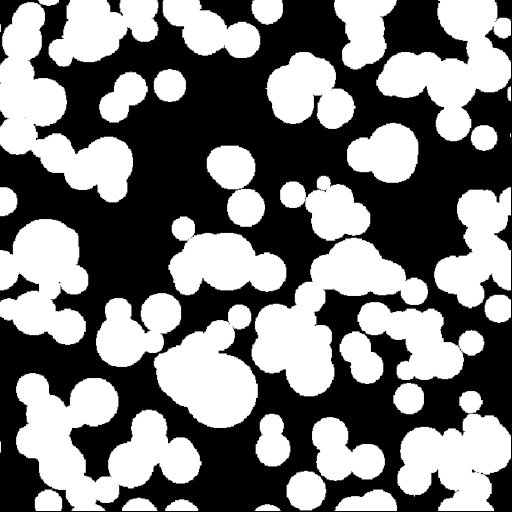
\includegraphics[scale=0.4]{inputs/512.png}
        \caption{The original image}
        \label{Fig.2a}
    \end{subfigure}
    \begin{subfigure}{.45\textwidth}
        \centering
        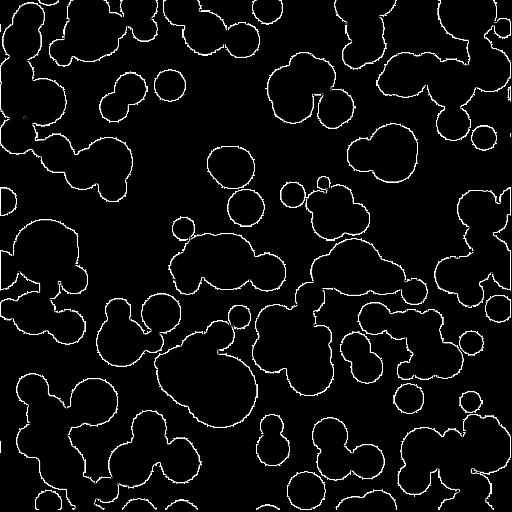
\includegraphics[scale=0.4]{output/512edge.png}
        \caption{After application of edge detection}
        \label{Fig.2b}
    \end{subfigure}
    \begin{subfigure}{.45\textwidth}
        \centering
        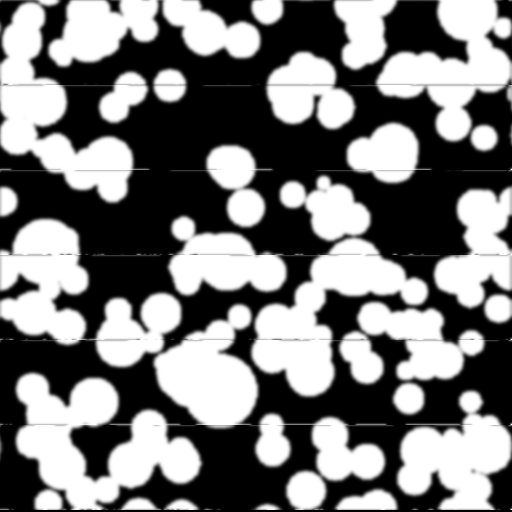
\includegraphics[scale=0.4]{output/512blur.png}
        \caption{After application of blur}
        \label{Fig.2c}
    \end{subfigure}
    \begin{subfigure}{.45\textwidth}
        \centering
        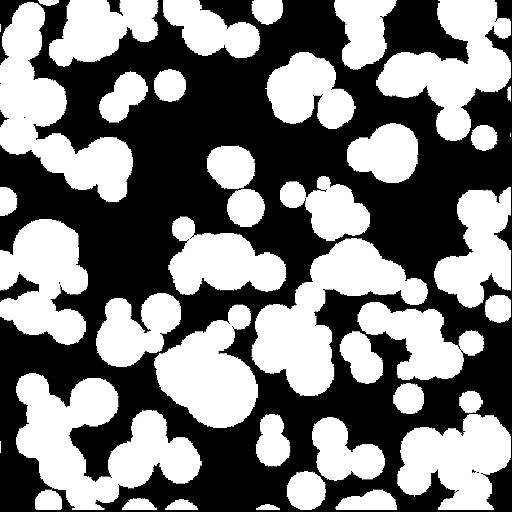
\includegraphics[scale=0.4]{output/512sharpen.png}
        \caption{After application of all three kernels}
        \label{Fig.2d}
    \end{subfigure}
    \caption{512 x 512 grayscale image}
    \label{Fig.2}
\end{figure}
\vfill
\newpage
The times measured for execution on the cluster are tabulated below. It could be 
construed from this table that the program exhibits marginal scalability.
\begin{table}[]
    \centering
    \begin{tabular}{lll}
    \textbf{\#P} & \textbf{With I/O} & \textbf{Without I/O} \\
    1            & 43.8              & 31.7                 \\
    2            & 36.7              & 28.0                 \\
    4            & 28.6              & 24.6                 \\
    6            & 27.8              & 24.5                 \\
    8            & 27.0              & 24.3                 \\
    12           & 26.6              & 24.0                 \\
    24           & 49.1              & 42.8                 \\
    36           & 125.7             & 61.2                
    \end{tabular}
    \caption{Measured times for different numbers of processes}
    \label{tab:time}
    \end{table}
\end{document}